
\chapter{Identification}
\label{cha:ident}
In this chapter, the identification process of the controlled system will be
explained. This identification process can be divided in two parts: the data acquisition, where the inputs\slash outputs of the system are
  acquired, and the model identification, where the acquired data is
  used in the identification algorithm, \Autoref{alg:identification}, and the
  identified model is generated.
  
In the next sections this two parts will be described

\section{Data Acquisition}
For the data acquisition, there are some ways to acquire the values of the
inputs\slash outputs, but most of them are divided in two categories, one where
the data is continuously registered, and the other one where the data is buffered
and registered in batches from time to time.
The first one is usually used for online processes, where the continuous flow of
information is necessary, and process that are repeated
extensively, examples of these processes are control loops and failure
detection modules. On the other hand, the second one usually serves for offline
processes, processes that are computationally expensive or happen only once in a
while. Modelling a big system and some more complex control loops can be examples of
such processes. 

Since the
\Autoref{alg:identification} takes as its input a set of paths, all the data is
acquired beforehand, a continuously acquisition is not necessary. The data can
be acquired in batches, and once all the data is collected the algorithm can be
run.

In order to acquire the data from a \PLC{}, the most straightforward way to do
it is by using datalogs. The Siemens \PLC{} S7-1500 includes function blocks to
use inside a \LD{} to store custom data in a \CSV{} formatted file. This file is
saved in a SD card. To retrieve this file, the SD card can be connected to a PC,
or it can be downloaded using a web browser if a Web Server is configured in the
\PLC.

The five blocks created to log data are called
\verb|DataLogCreate|,
\verb|DataLogOpen|, \verb|DataLogWrite|, \verb|DataLogClose| and \verb|DataLogDelete|.
They can be seen used in a \LD{} in \Autoref{fig:datalogcreate,fig:datalogopen,fig:datalogwrite,fig:datalogclose,fig:datalogdelete}.

The \verb|REQ| input in all blocks trigger the action to be performed in a
datalog: create the datalog file,
open it for writing, close it for writing, and deletes it, respectively.

The
\verb|ID| and \verb|NAME| inputs are the way to identify the datalog file, they
use a unique id number and a string. This string is used as the name of the
\verb|.csv| stored in the SD card.

The \verb|DATA| input is a struct that contains the data to be stored in the
\verb|.csv|. This struct can contain variables of different types even of
different sizes, for instance: it can contain a boolean,
an int, a word,
a string, and time.

The \verb|HEADER| input is a string to be \emph{prepended} to the first line of
the \verb|.csv| file, and it serves to identify each variable in the \verb|DATA|
input. As this string will be part of the \verb|.csv| file, it is needed to
include commas ``,'' inside it to separate the identifiers of the variables.

\begin{observation}
  \label{obs:stringSize}
 As string type has variable size, it is important to take into account its
 maximum size, that is $256$ Bytes, that means it can store up to 256 characters,
 considering the commas.
\end{observation}

The \verb|TIMESTAMP| input is a boolean that if it is $true$ the resulting
\verb|.csv| will have a timestamp column containing the time and date relative
to the time when the data line was inserted. 

\begin{figure}[H] \centering
 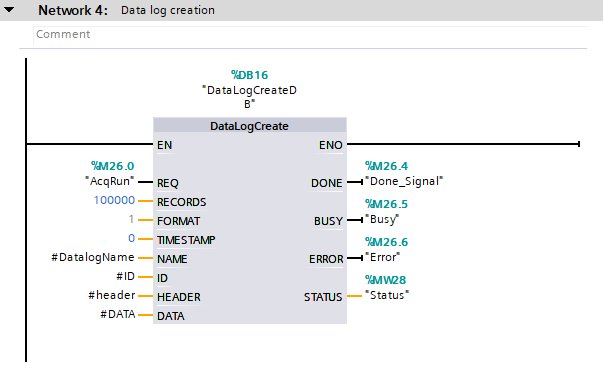
\includegraphics[width=0.7\textwidth]{tutorial/create}
  \caption{DataLogCreate block.}
  \label{fig:datalogcreate}
\end{figure}

\begin{figure}[H] \centering
 % \includegraphics[width=0.7\textwidth]{tutorial/datalogopen}
 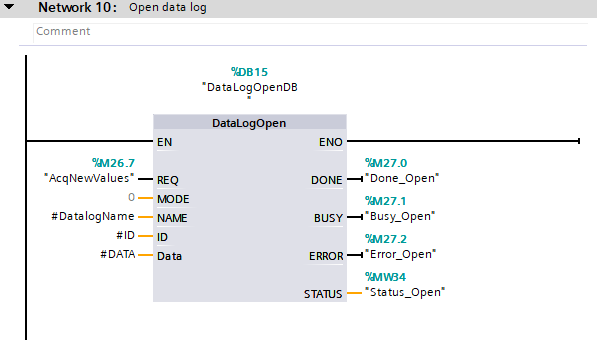
\includegraphics[width=0.7\textwidth]{tutorial/open}
\caption{DataLogOpen block.}
  \label{fig:datalogopen}
\end{figure}

\begin{figure}[H] \centering
	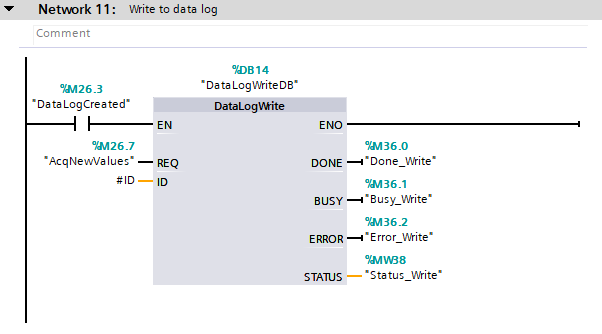
\includegraphics[width=0.7\textwidth]{tutorial/write}
	\caption{DataLogWrite block.}
	\label{fig:datalogwrite}
\end{figure}

\begin{figure}[H] \centering
 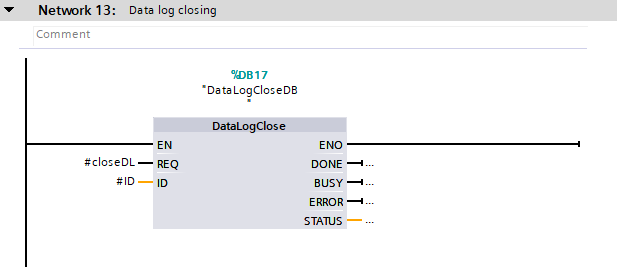
\includegraphics[width=0.7\textwidth]{tutorial/close}
  \caption{DataLogClose block.}
  \label{fig:datalogclose}
\end{figure}

\begin{figure}[H] \centering
 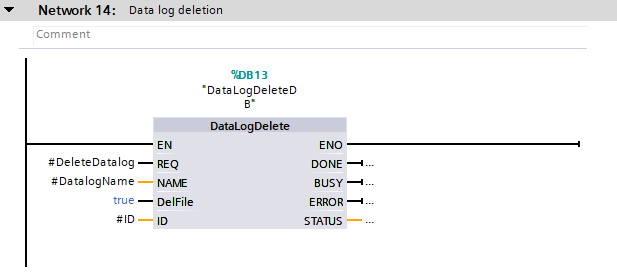
\includegraphics[width=0.7\textwidth]{tutorial/delete}
  \caption{DataLogDelete block.}
  \label{fig:datalogdelete}
\end{figure}
The outputs \verb|DONE|,\verb|BUSY|,\verb|ERROR| and \verb|STATUS| have as end
to identify the status of each block, bu they were not used in this work.

As a way to organise the data used for all these blocks, a \emph{DataBlock} was
used. The \Autoref{fig:exampleDataBlock} show the \emph{DataBlock} used and its
structure. We can see in it the main variables used to create
and write the log data: \verb|DATA|, \verb|HEADER|, \verb|ID| and \verb|NAME|.

More information about the blocks and its data can be seen in the Section 3.2 of
\cite{datalogSiemens}.

\begin{figure}[H] \centering
 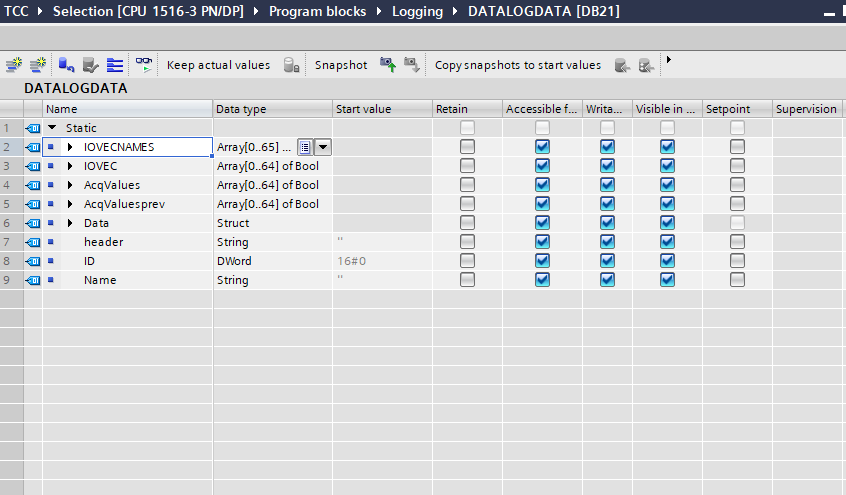
\includegraphics[width=\textwidth]{tutorial/datalog.png}
  \caption{Example of DataBlock used to log data.}
  \label{fig:exampleDataBlock}
\end{figure}

Since some of the needs of the identification process are not satisfied by
only using the blocks themselves, as a way to implement these needs, a block was created
that uses the datalog blocks together with others blocks, some of them are also
user-defined.

The needs of the identification process is to store the input\slash output
vectors of the controller, these being booleans, but store only when they
change, so there are never two consecutive lines with the same \emph{IOvector}.
Another need is to start and stop easily the acquisition, and even delete the
\verb|.csv| file.

The block created to satisfy these needs is called \emph{LOGDATA}. It can be seen in
\Autoref{fig:logdataBlock} and it has 12 inputs. The \verb|startAcq|,
\verb|stopAcq| and \verb|DeleteDL| inputs serve to start and stop the acquisition and
delete the \verb|.csv| file, respectively. The \verb|DatalogName| input serves
to give the name of the file. \verb|IOVECSIZE| tells the number of variables to
be stored. As one of the needs is to store only \emph{IOvectorss} different from its
adjacent vectors, it is needed to store the last \emph{IOvector} to compare it with a
new one just acquired, so enter the two inputs \verb|AcqValuesNew|,
\verb|AcqValuesPrev|. These two are arrays with size equivalent to the value
input in \verb|IOVECSIZE|. Their values are
changed from inside the block via an update block.
The \verb|IOVEC| is also an input that is changed from inside the block and it
is a temporary storage before it is sent to the variable connected to the
\verb|DATA| input, the latter input works exactly as the one shown in the
original blocks, this variable that is effectively stored in the file.

Instead of writing the name of the variables in the \verb|HEADER| input string,
as in the original blocks, a \verb|DATA_HEADERS| input is created. This input is
an array of size \verb|IOVECSIZE| that contains the names of all variables to be
stored in \verb|DATA|. These names are concatenated with
commas placed between them, and then this new string is assigned to the variable
in put in \verb|HEADER|, that is used as the header of the \verb|.csv|.
Remembering tha it is
very important to take observation \ref{obs:stringSize} on account.

\begin{figure}[H] \centering
 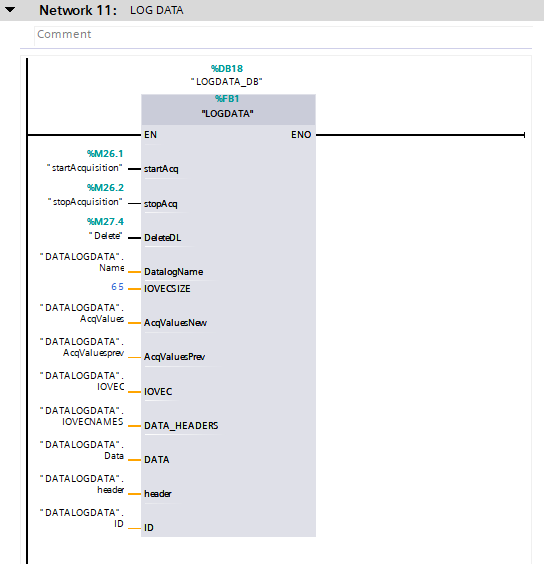
\includegraphics[width=0.7\textwidth]{tutorial/logdata.png}
  \caption{LOGDATA block.}
  \label{fig:logdataBlock}
\end{figure}

An example of the data stored in this work can be seen in
\Autoref{fig:exampleDataStruct}. As we can see the names of the variables inside the
struct \emph{Data} are the tags of the inputs and outputs of both \PLCs{} shown
in the \Autoref{sec:implementation}. 
\begin{figure}[H] \centering
 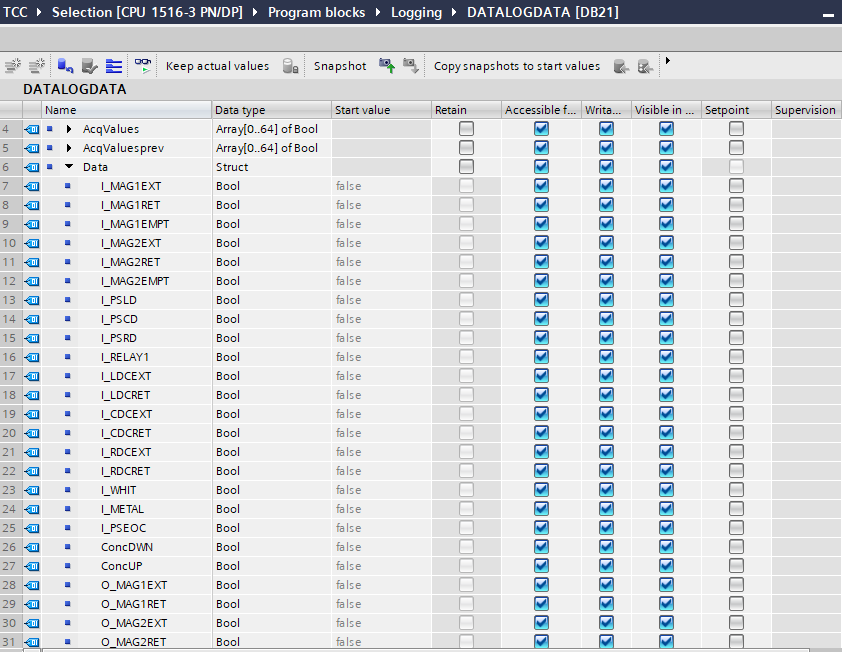
\includegraphics[width=\textwidth]{tutorial/datalogdata2.png}
  \caption{Example of Data struct.}
  \label{fig:exampleDataStruct}
\end{figure}

Inside this block some things are done in a certain order:
\begin{enumerate}
\item Copy \verb|AcqValuesNew| to \verb|AcqValuesPrev|
\item Update \verb|AcqValuesNew|
\item Compare \verb|AcqValuesNew| and \verb|AcqValuesPrev| 
\item prepare \verb|AcqValuesNew| to be stored (If different from \verb|AcqValuesPrev|) 
\item Create and open datalog if asked
\item Write the data if asked
\item Close and delete datalog if asked
\end{enumerate}

The last three steps are already depicted in
\Crefrange{fig:datalogcreate}{fig:datalogdelete}, the other ones will be shown
in the next paragraphs.


To Update the values of \verb|AcqValuesNew| the custom block called
\emph{UpdateValues} was created inside \emph{LOGDATA}. This block can be seen in
\Autoref{fig:updateValuesBlock}, and in \Autoref{fig:updateValuesBlockCode} we
can see the correspondence between the array and the tags.


\begin{figure}[H] \centering
 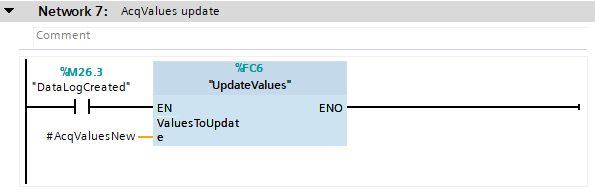
\includegraphics[width=0.7\textwidth]{tutorial/updateValues.png}
  \caption{UpdateValues block.}
  \label{fig:updateValuesBlock}
\end{figure}

\begin{figure}[H] \centering
 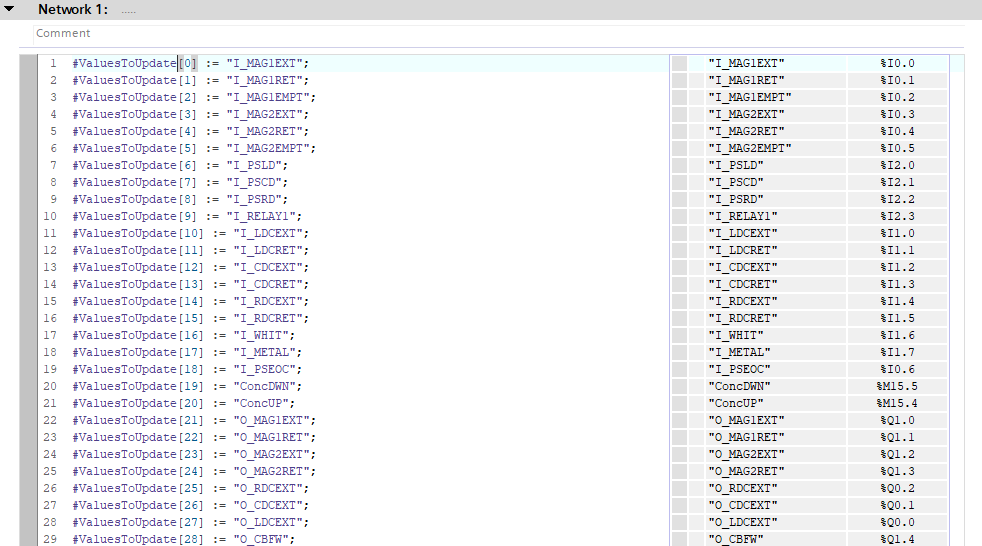
\includegraphics[width=\textwidth]{tutorial/updateValues2.png}
  \caption{Code inside UpdateValues block.}
  \label{fig:updateValuesBlockCode}
\end{figure}

In order to compare \verb|AcqValuesNew| and \verb|AcqValuesPrev|, a
\emph{CompareArrays} block was created where all the values are compared
bitwise, since they are booleans, and if they are different the
\verb|AcqValuesNew| is copied to the temporary variable input to \verb|IOVEC|.
This logic can be seen in \Autoref{fig:compareArrayBlock}.

\begin{figure}[H] \centering
 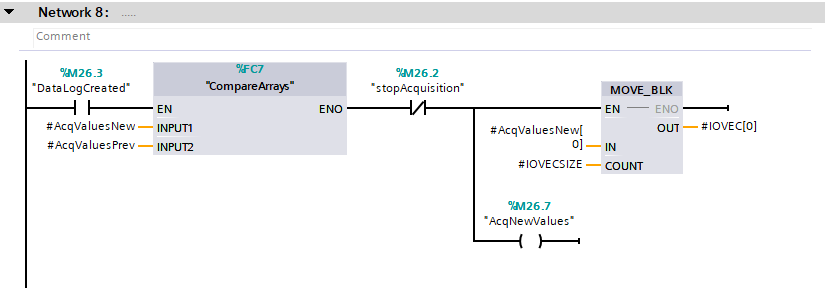
\includegraphics[width=\textwidth]{tutorial/compareArray}
  \caption{CompareArrays block.}
  \label{fig:compareArrayBlock}
\end{figure}

And just before storing the data using the blocks, the data in the temporary
variable \verb|IOVEC| is copied to \verb|DATA|, using the used defined block
\emph{PutInDataStruct} shown in \Autoref{fig:putInDataStructBlock} its content
can be seen in \Autoref{fig:putInDataStructBlockCode}.  

\begin{figure}[H] \centering
 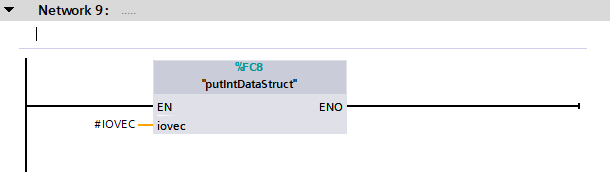
\includegraphics[width=0.7\textwidth]{tutorial/putindatastruct.png}
  \caption{PutInDataStruct block.}
  \label{fig:putInDataStructBlock}
\end{figure}

\begin{figure}[H] \centering
 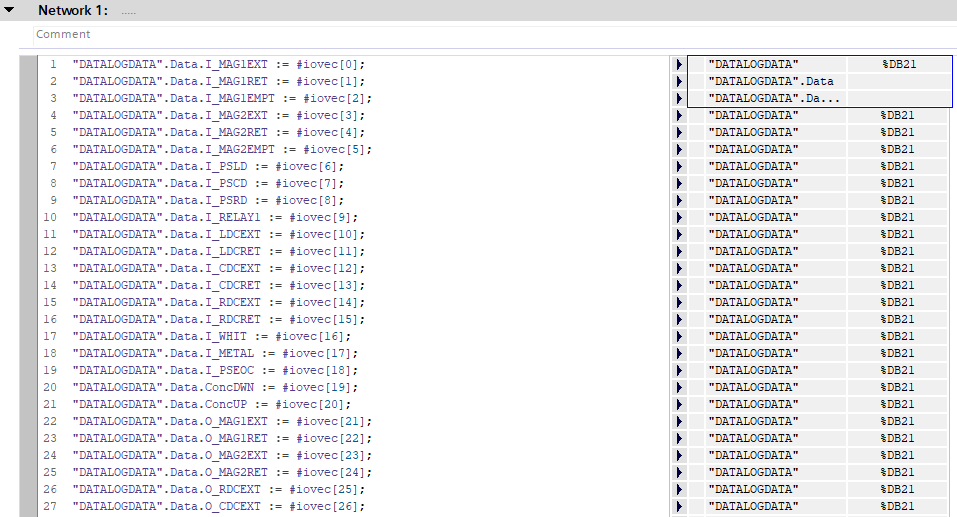
\includegraphics[width=\textwidth]{tutorial/putindatastruct2.png}
  \caption{Code inside PutInDataStruct block.}
  \label{fig:putInDataStructBlockCode}
\end{figure}

\begin{observation}
  Since the tags are divided between the 2 \PLCs{}, in order to have all tags in
  a same \PLC, ``Get'' and ``Put'' blocks were used along with a two Datablocks
  containing all the inputs and outputs of the Handling-Assembly-Storage \PLC.
  The aspect of these datablocks can be seen in \Autoref{fig:iovecFromPlc,fig:iovecFromPlctwo}
\end{observation}
\begin{figure}[H] \centering
\begin{subfigure}[h]{\textwidth} \centering
 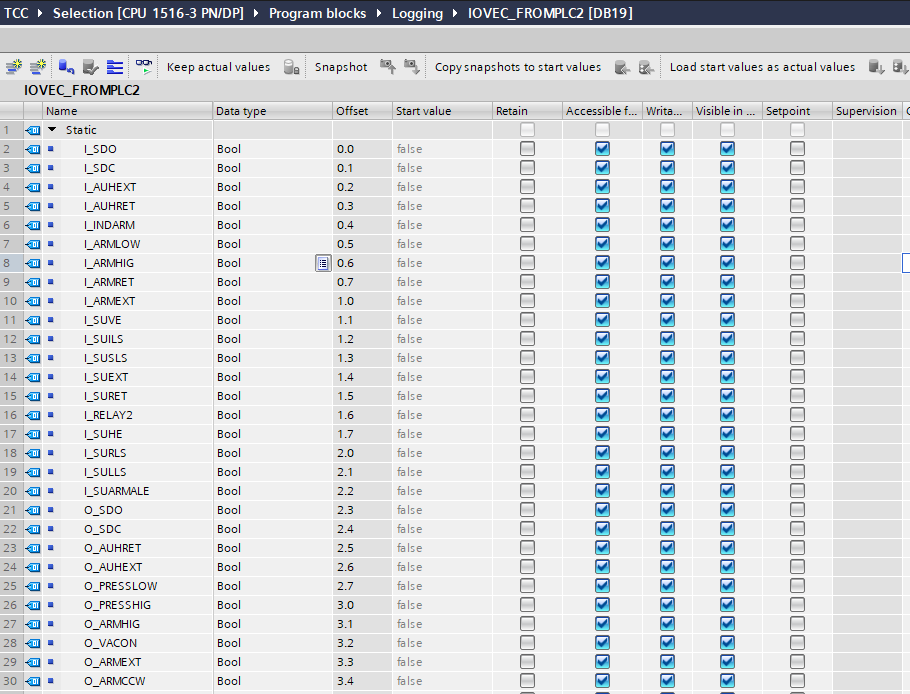
\includegraphics[width=\textwidth]{tutorial/iovecfromplc2.PNG}
  \caption{IOVEC\_FROMPLC2 DataBlock.}
  \label{fig:iovecFromPlc}
\end{subfigure}
\begin{subfigure}[h]{\textwidth} \centering
 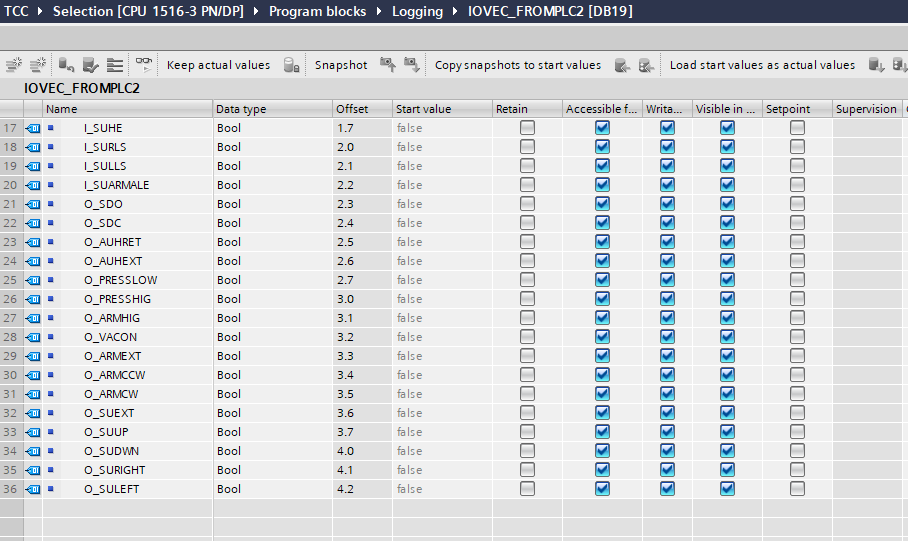
\includegraphics[width=\textwidth,clip,trim={0 1cm 0 0}]{tutorial/iovecfromplc2-1.PNG}
  \caption{IOVEC\_FROMPLC2 DataBlock - Continuing.}
  \label{fig:iovecFromPlctwo}
\end{subfigure}
\caption{Inputs\slash Outputs from Handling-Assembly-Storage \PLC.}
\end{figure}
% \subsection{HMI}
% \cite{webserverSiemens,userdefinedwebpagesSiemens}
% As a tool to facilitate the control of the system and the start and stop of acquisition, it was created a web page that is used as an  \HMI. It was created
% based on a bootstrap example\footnote{the example is available
%   at\url{https://getbootstrap.com/docs/4.3/examples/floating-labels/}}, and the
% html tags shown in the tutorial present in \cite{userdefinedwebpagesSiemens} using the a standard web page with the bootstrap buttons 

% \begin{figure}[H] \centering
%  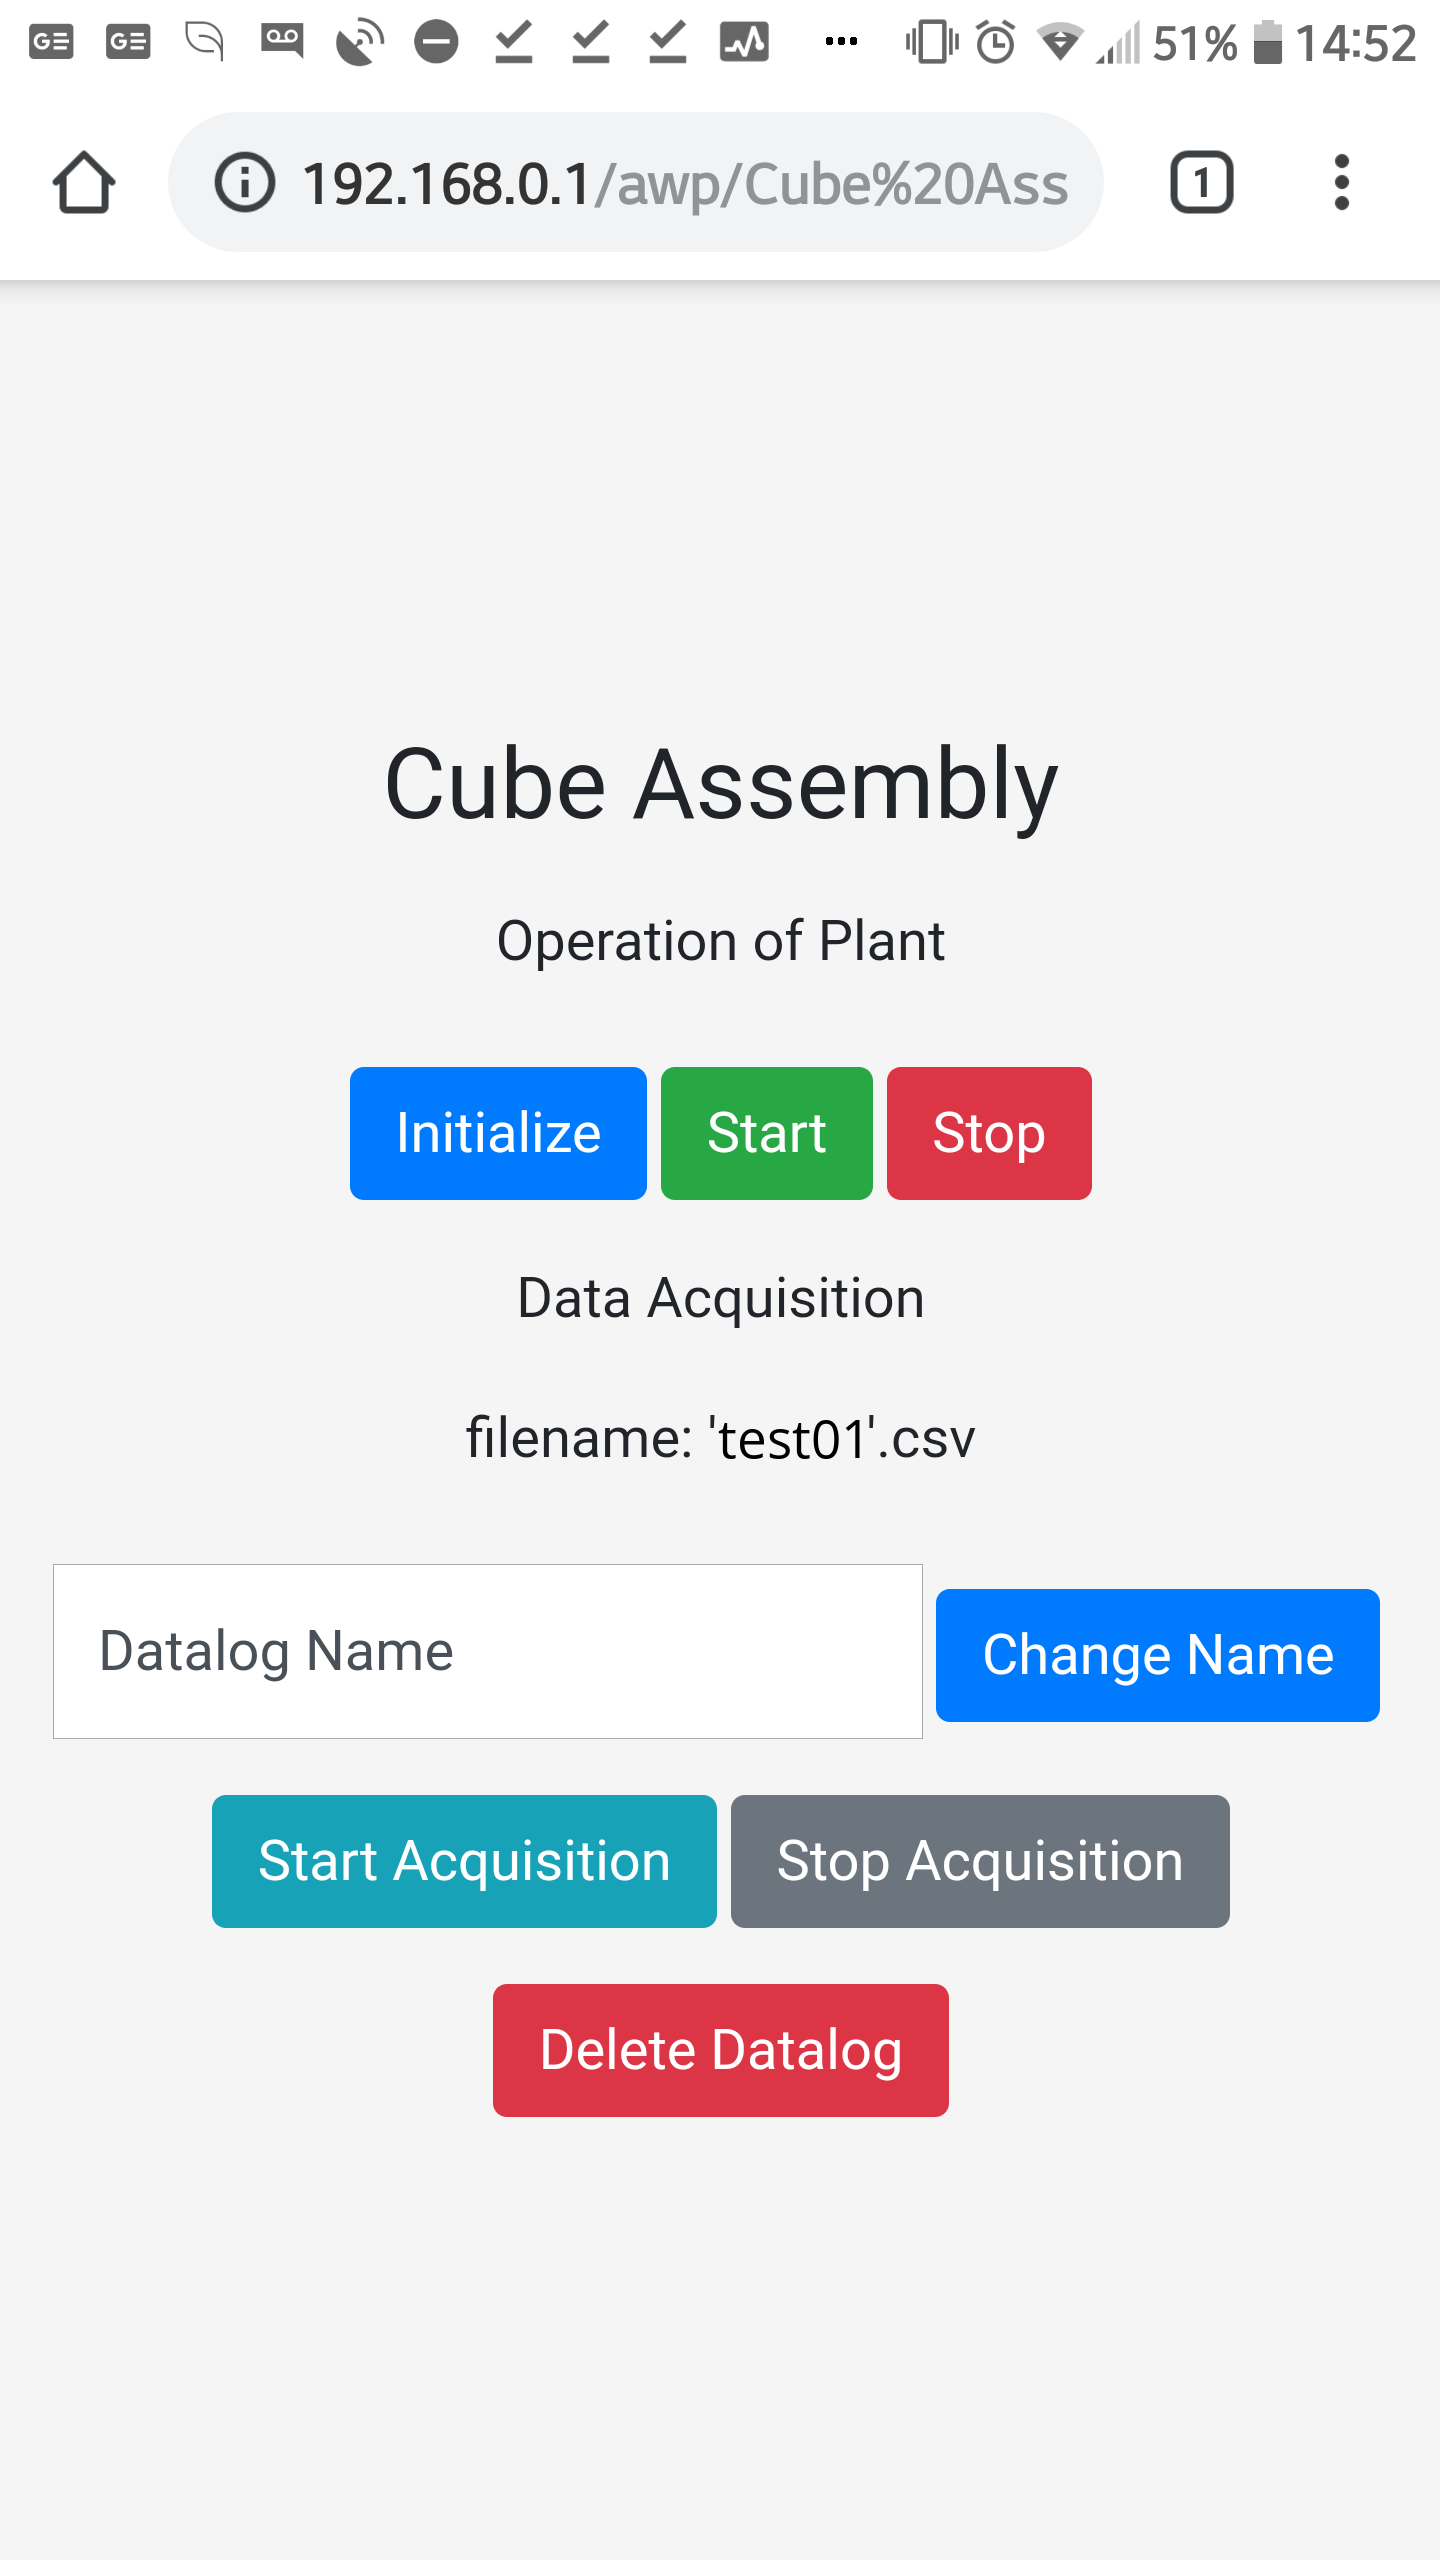
\includegraphics[height=0.6\textwidth]{hmi_mobile2}
%   \caption{HMI on mobile.}
%   \label{fig:hmi_mobile}
% \end{figure}
\begin{observation}
  Since this is the first version of the block, that are still lots of
  improvements to be made to optimise its use. Some variables can be changed, in
  order to be used as 
  internal variables, instead of creating new variables in a DataBlock. And
  maybe some variables and even rungs can be removed or substituted.
\end{observation}
\section{Model Identification}
As said previously, once the data is logged, the \verb|.csv| file can be downloaded from a Web Server, if
this one is configured, or from the SD card. Simply following the steps shown in
\cite{webserverSiemens}, it is possible to configure a web server in the Siemens
\PLC S7-1500. And once it is configured, the file can be downloaded in different
ways, most of them are shown in section 3.13 of \cite{webserverSiemens}. Two of
them are by clicking
the download button shown in the DataLogs web page or by a bash script, as the following: \newline
\verb|wget --content-disposition -i "http://192.168.2.132/DataLogs?Action=LIST"|.
The address ``192.168.2.132'' should be changed by the address of the \PLC{} in which
the web server is running.

When the \verb|.csv| is already copied to a PC, the identification algorithm can
be run. This identification algorithm, \Autoref{alg:identification}, was
implemented in python, but as the algorithm takes modified paths as input, the paths
are needed to be extracted from the \verb|.csv| and then modified using the
\Autoref{eq:modifiedPath,eq:modifiedPathb}, also implemented in ptyhon. As the identification is
made using a black box approach, we do not have any previous information of what is
considered a path in the file, so the first vector is considered as the initial
vector, and every time it is repeats another branch is created.

So, as an example, if we had the observed data of the example from
\cite{moreira2018enhanced}, the one shown in \Autoref{sec:identification}, in a
\verb|.csv| file, instead of 3 paths, as shown in the example, 4 paths would be
created, as follows:
\setlength\arraycolsep{2pt}
\begin{align*}
  p_1&= \left(\colvec{1\\0\\0},a,\colvec{1\\1\\0},b,\colvec{0\\1\\1},c,\colvec{0\\0\\0},d,\colvec{0\\0\\1},e,\colvec{1\\0\\0}\right) \\
  p_2&= \left(\colvec{1\\0\\0},g,\colvec{0\\0\\0},h,\colvec{1\\1\\0},b,\colvec{0\\1\\1},c,\colvec{0\\0\\0},i,\colvec{1\\0\\0}\right) \\
  p_3&= \left(\colvec{1\\0\\0},j,\colvec{0\\1\\1},l,\colvec{1\\0\\0}\right) \\
  p_4&= \left(\colvec{1\\0\\0},g,\colvec{0\\0\\0},h,\colvec{1\\1\\0},b,\colvec{0\\1\\1},i,\colvec{1\\1\\1},m,\colvec{0\\0\\0},d,\colvec{0\\0\\1},n,\colvec{1\\1\\0}\right) \\
\end{align*}
If we compare these paths with those shown in \Autoref{sec:identification},
we can see that $p_3$ of this section is part of $p_2$ from
\Autoref{sec:identification}. This change in number of paths is reflected on the
identified model. Running the identification algorithm with the extracted paths and using
the same parameters, $k=1$ and $k=2$, it was possible to identify the state
transition diagrams seen in \Autoref{fig:identExamplekone,fig:identExamplektwo}.
Comparing them with \Autoref{fig:examplek1,fig:examplek2}, we can see the difference
caused by the additional path in the identified model. A brief discussion about
the way the paths are chosen will be made in \Autoref{cha:results}.

\begin{figure}[H]
  \centering
  \includegraphics[width=\textwidth]{example/examplek1NoArrows}
  % \includetikzfigure[width=\textwidth]{example/stdin}
  \caption{Identified model from paths extracted from \texttt{.csv} file using $k=1$.}
  \label{fig:identExamplekone}
\end{figure}

\begin{figure}[H]
  \centering
  \centering
  \includegraphics[width=\textwidth]{example/examplek2NoArrows}
  % \includetikzfigure[width=\textwidth]{example/examplek2}
  \caption{Identified model from paths extracted from \texttt{.csv} file using $k=2$.}
  \label{fig:identExamplektwo}
\end{figure}
The tools created to implement the extraction of the paths and the
identification algorithm will be commented in \Autoref{sec:daoct}, together with
other useful tools used in this work.


%%% Local Variables:
%%% mode: latex
%%% TeX-master: "../monografia"
%%% End: